\section{Potential and actual infinity}

% The work of \textcite{Lak00} provides a wide range of examples of
% metaphorical reasoning in mathematics, while stressing the embodied
% cognition involved in basic mathematical experience.  

Some of the ideas of \textcite{Lak00} have been reworked by the
authors, with increased emphasis on conceptual blending.
In particular, the analysis of mathematical infinity, given in
metaphorical form as the ``Basic Metaphor of Infinity'' (BMI) in
\textcite{Lak00}, is represented in blend form in \textcite{nunez05}
as the ``Basic Mapping of Infinity'' (so, still ``BMI'').

We show here how this blend works out in our setting.
The BMI suggests that the notion of completed infinity,
in particular the possibility of transfinite numbers in the sense
of Cantor, comes from a blend of the notion of completed,
finite process with that of a potentially infinite and endless
process.

Thus take two corresponding input spaces, given by CASL specifications
\textbf{FinEnd} and \textbf{Inf} corresponding to the following diagrams


  \noindent
  \textbf{FinEnd:}
\begin{center}
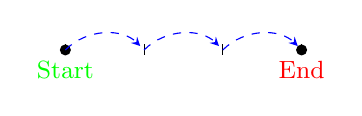
\begin{tikzpicture}[out=45,in=135,relative,>=stealth]
  \foreach \x in {0,...,3} \draw[shift={(\x,0)},color=black] (0pt,2pt)
  -- (0pt,-2pt);% node[below] {\footnotesize $\x$};
  \fill (0,0) circle (2pt); \fill (3,0) circle (2pt);

  \draw[dashed,->,color=blue,shorten >=2pt]{(0,0) to (1,0)};
  \draw[dashed,->,color=blue,shorten >=2pt]{(1,0) to (2,0)};
  \draw[dashed,->,color=blue,shorten >=2pt]{(2,0) to (3,0)};

  \node[color=red] at (3,-0.25) {\small End}; \node[color=green] at
  (0,-0.25) {\small Start};

\end{tikzpicture}
\end{center}
\noindent\textbf{Inf:} 
\begin{center}
  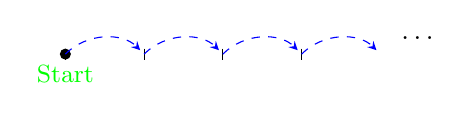
\begin{tikzpicture}[out=45,in=135,relative,>=stealth]
    \foreach \x in {0,...,3} \draw[shift={(\x,0)},color=black]
    (0pt,2pt) -- (0pt,-2pt); \fill (0,0) circle (2pt);
    % \fill (3,0) circle (2pt);

    \draw[dashed,->,color=blue,shorten >=2pt]{(0,0) to (1,0)};
    \draw[dashed,->,color=blue,shorten >=2pt]{(1,0) to (2,0)};
    \draw[dashed,->,color=blue,shorten >=2pt]{(2,0) to (3,0)};
    \draw[dashed,->,color=blue,shorten >=2pt]{(3,0) to (4,0)};

    \node at (4.5,0.2) {\dots}; \node[color=green] at (0,-0.25)
    {\small Start};

  \end{tikzpicture}
\end{center}

% \begin{figure}[h]
%   \centering
% 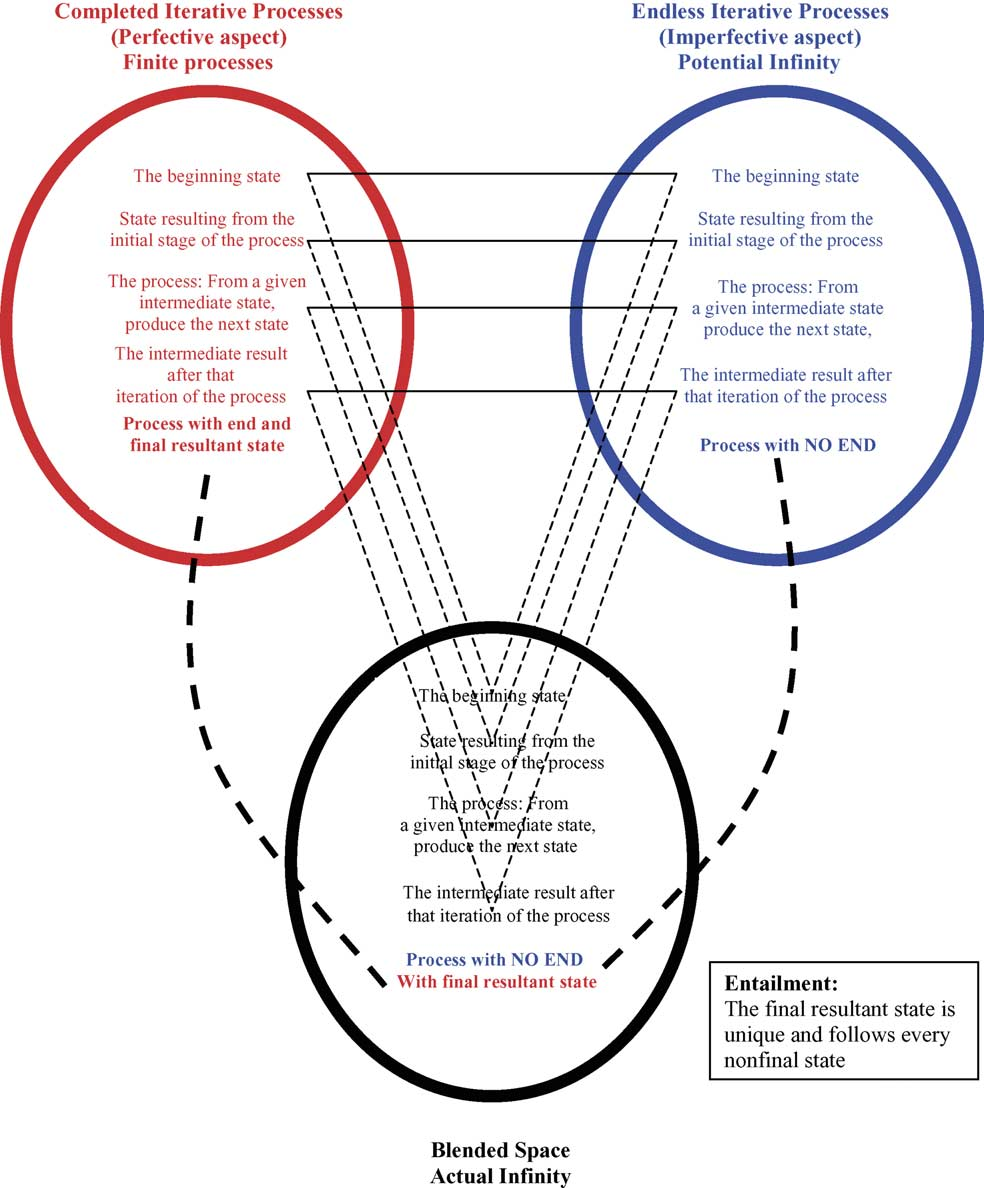
\includegraphics[width=0.4\textwidth]{transfin_nunez}  
%   \caption{Blend from \textcite[p ??]{nunez05}}
%   \label{fig:nunez_transfin}
% \end{figure}

% Figure~\ref{fig:nunez_transfin} gives an indication of the components
% of the blend:
\begin{itemize}
\item  \textbf{FinEnd:} Completed Iterative Processes
are those that from some initial state, terminate in a final state
after a finite number of state transitions.  One such case is chosen.
\item 
\textbf{Inf:} Infinite Iterative Processes are those that continue indefinitely
to change state.
\end{itemize}
In both cases, the arrows indicate steps of the processes, and
the process states are in a discrete linear order indicated by left-to-right
order in the diagrams.

The generic space \textbf{Gen} simply identifies the start states, the
notion of process step, and the linear ordering of states.

Now we can compute the blend of these spaces,
which includes new features taken from both of the
input spaces.  This blend is \emph{inconsistent}, for the
following two reasons:
\begin{enumerate}
\item the number of states is finite (from \textbf{FinEnd}), and infinite
(from \textbf{Inf});
\item  there both is an end state (from \textbf{FinEnd})
and is no end state (from \textbf{Inf}).
\end{enumerate}
Search through the possibilities of weakening the input spaces by
omitting as few axioms as possible among those involved
in an inconsistency reveals the possibility of a structure
with infinitely many states (from \textbf{Inf}) and an
end state (from \textbf{FinEnd}).  Computing the
colimit from the weakened input spaces \textbf{W-FinEnd}, \textbf{W-Inf}
gives a theory corresponding to this diagram:
\begin{center}
  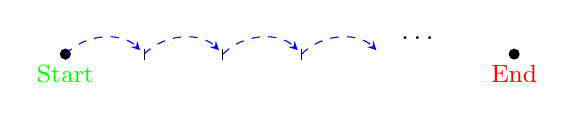
\begin{tikzpicture}[out=45,in=135,relative,>=stealth]
    \foreach \x in {0,...,3} \draw[shift={(\x,0)},color=black]
    (0pt,2pt) -- (0pt,-2pt); \fill (0,0) circle (2pt); \fill (5.7,0)
    circle (2pt);
    % \fill (3,0) circle (2pt);

    \draw[dashed,->,color=blue,shorten >=2pt]{(0,0) to (1,0)};
    \draw[dashed,->,color=blue,shorten >=2pt]{(1,0) to (2,0)};
    \draw[dashed,->,color=blue,shorten >=2pt]{(2,0) to (3,0)};
    \draw[dashed,->,color=blue,shorten >=2pt]{(3,0) to (4,0)};

    \node at (4.5,0.2) {\dots}; \node[color=green] at (0,-0.25)
    {\small Start}; \node[color=red] at (5.7,-0.25) {\small End};

  \end{tikzpicture}
\end{center}
Thus we have a blend as in the earlier examples:

%\begin{center}
%  \begin{tikzcd}[column sep=normal, row sep=small]
%    & \textrm{Colimit}
%    \\
%    \SIdIndex{W-FinEnd} \arrow{ur}{} & & \SIdIndex{W-Inf} \arrow{ul}[swap]{} \\
%    & \textrm{Gen} \arrow{ul}{}
%    \arrow{ur}[swap]{}
%  \end{tikzcd}
%\end{center}
\begin{center}
  \begin{tikzcd}[column sep=small, row sep=tiny]
    & \textrm{Colimit}
    \\
    \SIdIndex{W-FinEnd} \arrow{ur}{} & & \SIdIndex{W-Inf} \arrow{ul}[swap]{} \\
    & \textrm{Gen} \arrow{ul}{}
    \arrow{ur}[swap]{}
  \end{tikzcd}
\end{center}

   % On the other hand, if we interprete the conceptual spaces from a             
   % topological perspective \parencite{munkrestopology}, where
   % different states are in a topological space, then, the resulting       
   % blend can be clearly seen as the one-point compactification of a
   % potential infinite topological space, where the final state                
   % corresponds to the point at the infinity.


%%% Local Variables: 
%%% mode: latex
%%% TeX-master: "mathsICCC"
%%% End: 
